
\documentclass[11pt]{article}

\usepackage{common}
\usepackage{hyperref}
\title{HW2: NLP From Scratch}
\author{Alexander Rush \\ srush@seas.harvard.edu \and Sam Wiseman \\ swiseman@seas.harvard.edu }
\begin{document}

\maketitle{}
\section{Introduction}

In this assignment, we tackle the problem of part-of-speech tagging. 

The problem can be outlined as follows. Given a set of tokenized text with each token given a tag corresponding to the part of speech that it functions as, can we train a model that can read in other sets of tokenized text and accurately determine the part of speech for every word? 

We will train our models on a tagged excerpt from the Wall Street Journal and test them on another. We examine three different models for this purpose. These three models are multinomial naive Bayes, logistic regression, and the neural network from [Collobert et al]. 

In Section $2$, we introduce our notation and give a description of our problem in formal language. In Section $3$, we describe our three models. In Section $4$, we present our experimental results for model performance and hyperparamater tuning. In Section $5$, we conclude with a discussion of our results. 

\section{Problem Description}

Our raw data consists of pairs $(w_i, t_i)$, where $w_i$ is a word and $t_i$ is its corresponding part of speech tag. The $t_i$ are elements of a finite set of classes $\mcT$, which we take as the list of POS tags provided in the homework. Example tags are NNP, VBD, VBZ, etc. and in this problem we have a total of $|\mcT| = 45$ tags.

We construct a feature representation $\phi(w_i)$ of each word as follows. 

First, construct the vocabulary $\mcV$ of the training and testing sets. To keep this from growing too large, we only use lower-case words. Furthermore, we map any uncommon words to a special ``RARE'' word, where we use the words in the publicly available data from [Glove paper] as our ``common words'' dictionary. Then, we can associate a sparse one-hot feature vector $j_i \in \{0,1\}^{|\mcV|}$ to word $w_i$ that represents the index $j$ that $w_i$ maps to in $\mcV$.

Second, we can also construct a sparse one-hot feature vector $c_i \in \{0,1\}^c$ that keeps track of the capitalization information in $w_i$ that we lost above. This tracks whether $w_i$ is all uppercase, all lowercase, starts with an uppercase letter, contains an uppercase letter, or satisfies none of these conditions. 

Finally, we add context by not only adding in the features of $w_i$ to $\phi(w_i)$, but also adding in the features of the words in a \emph{window} around $w_i$. In our case, we use a window of size $5$, so $\phi(w_i)$ consists of vectors $\boldx_{word} = \{j_{i-2}, j_{i-1},j_i, j_{i+1}, j_{i+2}\}$ and $\boldx_{cap} = \{c_{i-2}, c_{i-1}, c_i, c_{i+1}, c_{i+2}\}$ of vocabulary and capitalization features corresponding to the surrounding word window, which we will denote by $\boldw_i$ or $\boldw$ for short. 

Our goal is to learn a function $f: (\{0,1\}^{|\mcV|} \times \{0,1\}^c) \to [0,1]^\mcT$ that takes in a window of words $\boldw$ and outputs a prediction vector $\hat{\boldy}$ where $\hat{y}_k$ is the probability $p(k|w_3)$ of the middle word $w_3 \in \boldw$ having tag $k$.

\subsection{Extension: Suffix Features}

As an extension to the baseline model described in Collobert et al, we add in suffix features as well. %%%

\section{Model and Algorithms}

We use three models:
\begin{itemize}
  \item multinomial naive Bayes (MNB)
  \item logistic regression
  \item neural network from [Collobert]
\end{itemize}

Below we describe the setup of each.

\subsection{Multinomial Naive Bayes}

In MNB, we assume that the features of a word window $\boldw$ are independent of each other. 

We can apply Bayes' law to calculate the probability $p(t| \boldw)$ of class $t$ given $\boldw$. 
$$p(t| \boldw) = \frac{p(t)p(\boldw |t)}{p(\boldw)}$$

Our prediction $\hat{y}$ for $\boldw$ is given by the maximum-probability tag
$$\hat{y} = \argmax_{t} p(t | x)$$

Note that $\boldw$ is a window of words. Assuming that the middle word is equal to $w_i$, we can apply our independence assumption to get 

$$p(t | \boldw) = \frac{p(t)\prod_{d=-2}^{d=2} p(w_{i+d} | t)}{\prod_{d=-2}^{d=2} p(w_{i+d})}$$

The $p(w_{i+d})$ are constant functions of the output $t$, so we can focus on calculating the terms in the numerator. 

Recall that every word $w$ can be represented as a two sets of binary values $e_1, \dots, e_{|\mcV|}$ and $e^{cap}_1, \dots, e^{cap}_{|c|}$. By our independence assumption, we have 
$$p(w | t) = p(e_1, \dots, e_{|\mcV|}, e^{cap}_1, \dots, e^{cap}_{|c|} | t) = \prod_{m=1}^{|\mcV|} p(e_m | t) \prod_{n=1}^{|c|} p(e^{cap}_n | t)$$

Therefore, it suffices to maximize the $p(e_m | t)$ and $p(e^{cap}_n | t)$. Under negative log-likelihood loss, these are maximized over the entire training set by counting the number of samples with tag $t$ that have word feature $e_m$ and capitalization feature $e^{cap}_n$ respectively and then dividing by the total number of samples with tag $t$. 

The maximum likelihood estimate for $p(t)$ is the proportion of samples with tag $t$. 

Overall, our prediction becomes
$$\hat{y} = \argmax_t \sum_d (\sum_m \log p(e_m | t) + \sum_n \log p(e^{cap}_n | t)) + \log p(t)$$
where the sum is taken over all words in the window $\boldw$. 

\subsection{Logistic Regression}

We assume a linear model $z = \boldx_{word} \boldW + \boldx_{cap} \boldW_{cap} + \boldb$, where $\boldx_{word}$ and $\boldx_{cap}$ are the word and capitalization features of an input word window $\boldw$. 

We then apply the softmax function to get an output $\hat{\boldy}$, where $\hat{y}_t$ is the predicted probability for a tag $t$ given the window $\boldw$. 

This is implemented using the following neural network architecture:
(Picture)

where the gradients are optimized via stochastic gradient descent like in our last assignment. 

\subsection{Neural Network}

\begin{itemize}
\item diagrams of your model,

  \begin{center}
    \includegraphics[width=0.4\textwidth]{network}
  \end{center}
\item feature tables,

  \begin{center}
    \begin{tabular}{@{}lll@{}}
      \toprule
      &\multicolumn{2}{c}{Mention Features  } \\
      & Feature & Value Set\\
      \midrule
      & Mention Head & $\mcV$ \\
      & Mention First Word & $\mcV$ \\
      & Mention Last Word & $\mcV$ \\
      & Word Preceding Mention & $\mcV$ \\
      & Word Following Mention & $\mcV$\\
      & \# Words in Mention & $\{1, 2, \ldots \}$ \\
      & Mention Type & $\mathcal{T}$ \\
      \bottomrule
    \end{tabular}
  \end{center}

\item pseudo-code,

  \begin{algorithmic}[1]
    \Procedure{Linearize}{$x_1\ldots x_N$, $K$, $g$}
    \State{$B_0 \gets \langle (\langle \rangle, \{1, \ldots, N\}, 0, \boldh_0, \mathbf{0})  \rangle$}
    \For{$m = 0, \ldots, M-1$ }
    \For{$k = 1, \ldots, |B_m|$}
    \For{$i \in \mcR$}
    \State{$(y, \mcR, s, \boldh) \gets \mathrm{copy}(B_m^{(k)})$}
    \For{word $w$ in phrase $x_i$}
    \State{$y \gets y $ append $w$ }
    \State{$s \gets s + \log q(w, \boldh) $ }
    \State{$\boldh \gets \delta(w, \boldh)$}
    \EndFor{}
    \State{$B_{m+|w_i|} \gets B_{m+|w_i|} + (y, \mcR - i, s,   \boldh)$}
    \State{keep top-$K$ of $B_{m+|w_i|}$ by $f(x, y) + g(\mcR)$}
    \EndFor{}
    \EndFor{}
    \EndFor{}
    \State{\Return{$B_{M}^{(k)}$}}
    \EndProcedure{}
  \end{algorithmic}

\end{itemize}

\subsection{Training Methods}

We ran vanilla batch stochastic gradient descent on training and validation sets. For batches, we shuffled the training set once and iterated over it for each epoch. For preliminary results we ran SGD for at least 5 epochs, and then stopped when relative validation loss (defined as the fractional change in validation loss) dropped below $0.1\%$.

We continued training on the neural model (with Glove word embeddings) when it was clear that the model had not completed training with this criterion. The use of validation error rather than training error prevents overfitting.

\section{Experiments}

We ran batch SGD for maximum 20 epochs with batch size 32 and learning rate 0.01. For naive Bayes we used $\alpha = 1$. For neural models, we used word embedding dimension 50, capitalization feature embedding dimension 5, and hidden layer size 300 (as in Collobert et al). We ran most experiments on Odyssey with 16GB memory.

Training time tended to vary for each model depending on the Odyssey server it ran on and time of day. Table~\ref{tab:timings} gives some ballpark timing results for each model.

\begin{table}[h]
\centering
\begin{tabular}{llr}
 \toprule
 Model &  & Timing \\
 \midrule
 \textsc{Naive Bayes} & & 16 s\\
 \textsc{Logistic Regression (per epoch)} & & 10 min \\
 \textsc{Neural (per epoch)} & &12 min \\
 \bottomrule
\end{tabular}
\caption{\label{tab:timing} Timing results on PTB training.}
\end{table}

%For the PTB dataset, which has 950885 training points, a batch size of 32 gives a training time of 

Figure ~\ref{fig:loss} shows the training and validation loss over epochs for the neural model with Glove word embeddings. Note that loss consistently decreases, and we stopped training when validation loss stopped decreasing. The bump in the validation accuracy is from when we restart training, and is possibly due to a new batch shuffle.

\begin{figure}
	\centering
	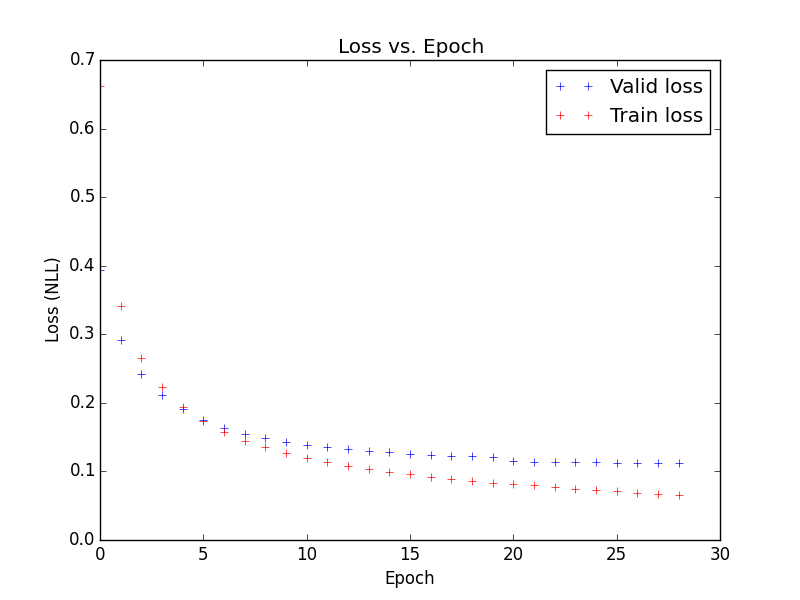
\includegraphics[scale=0.4]{loss_plots}
	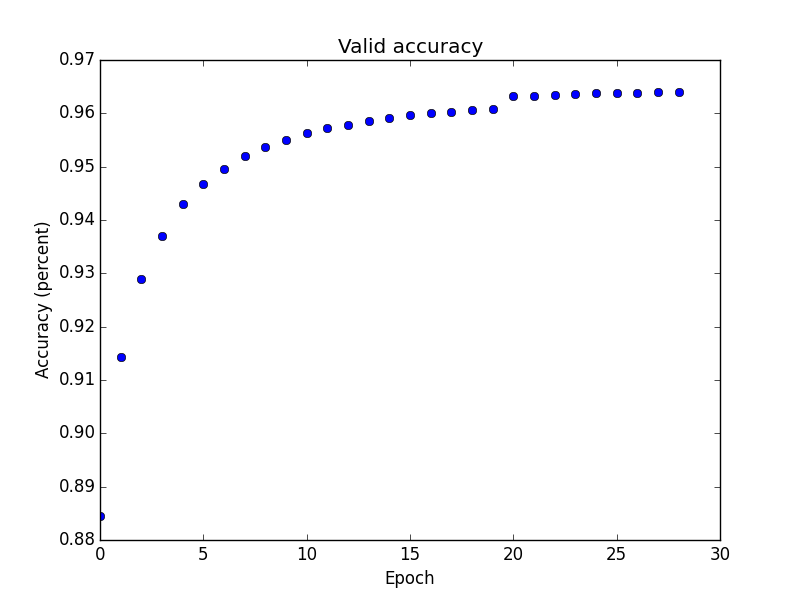
\includegraphics[scale=0.4]{acc_plot}
	\caption{\label{fig:loss} Training curves.}
\end{figure}

We found that after 20 epochs, the neural model with pretrained word embeddings had the best validation rate, but training had not yet converged. Thus, we ran it for about 10 more epochs until the validation error stopped decreasing.

Table~\ref{tab:results} gives the classification accuracy of each model on the validation set. The results shown are after training 20 epochs, except for models with Glove embeddings (which we trained for longer). For neural models, GLOVE means we used pretrained Glove word embeddings and SUFF means we included suffix features.

\begin{table}[h]
\centering
\begin{tabular}{llr}
 \toprule
 Model &  & Acc. \\
 \midrule
 \textsc{Naive Bayes} & & 91.27\\
 \textsc{Naive Bayes (w/o capitalization)} & & 89.98 \\
 \textsc{Logistic Regression} & & 76.50 \\
 \textsc{Neural} & & 92.11  \\
 \textsc{Neural+GLOVE} & &96.41 \\
 \textsc{Neural+GLOVE+SUFF} & & ??? \\
 \bottomrule
\end{tabular}
\caption{\label{tab:results} Results on PTB POS tagging.}
\end{table}

As an extension, we also tried to run Adadelta instead of SGD. However, because it saves $O(P)$ values where $P$ is the number of parameters in the model, it turns out to be prohibitively expensive for memory, and training did not finish in time.

\section{Conclusion}

In this homework...

We found that training these neural models takes a significant amount of time, and thus careful logging and saving models after each epoch was important. Running on Odyssey also helped by offloading computation to a cloud server. We expect that with GPUs, training these models will be much quicker and easier.

The code for this homework can be found here: \url{https://github.com/r0hilp/cs287-hw2}

\bibliographystyle{apalike}
\bibliography{writeup}

\end{document}
